% ansatz 3
\section{AnonAccess}

%----------------------------------------------------------

\begin{frame}
	\frametitle{AnonAccess}
	Zusätzliche Datenbank für Änderungen
	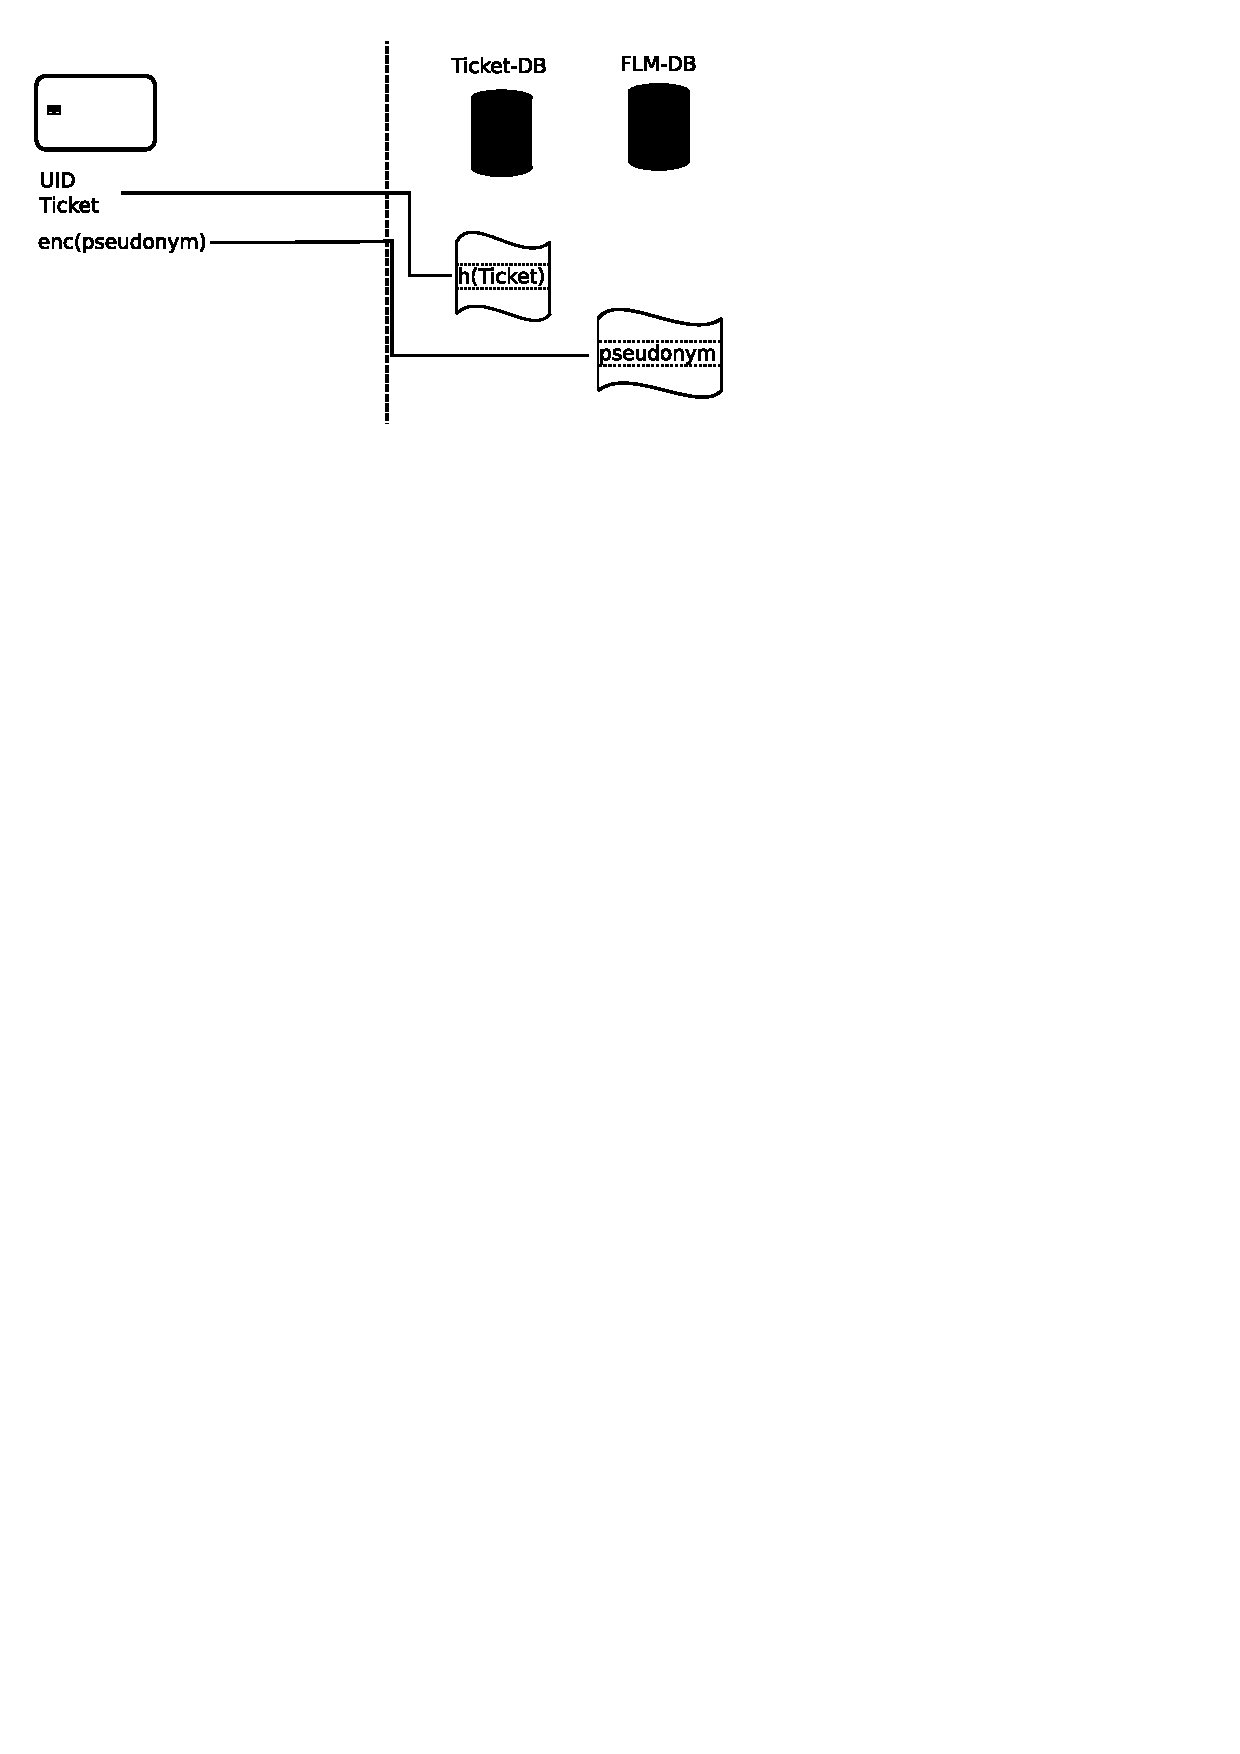
\includegraphics[scale=0.75]{ansatz3.pdf}
\end{frame}

%----------------------------------------------------------

\begin{frame}
	\frametitle{AuthBlock Struktur}
%typedef struct{
%	uid_t    uid;
%	ticket_t ticket;
%	uint8_t  rkey[32];
%	uint8_t  rid[32];
%	uint8_t  pinhmac[32];
%	uint8_t  hmac[32];
%} authblock_t;
\begin{tabular}{|c|c|}
\hline UID & User ID; Index in die Ticket-DB \\ 
\hline Ticket   & $enc_{TicketKey}(24 Byte Zufall \parallel 8 Byte Zeitstempel)$ \\ 
\hline rkey     & 32 Byte zufälliger Schlüssel \\ 
\hline rid      & $enc_{ridKey}(enc_{rkey}(Pseudonym))$ \\ 
\hline HMAC     & HMAC über die vorrangegangenen Daten \\ 
\hline 
\end{tabular} 
\end{frame}

%----------------------------------------------------------

\begin{frame}
	\frametitle{AuthBlock Struktur}
%typedef struct{
%	uid_t    uid;
%	ticket_t ticket;
%	uint8_t  rkey[32];
%	uint8_t  rid[32];
%	uint8_t  pinhmac[32];
%	uint8_t  hmac[32];
%} authblock_t;
\begin{tabular}{|c|c|}
\hline UID & User ID; Index in die Ticket-DB \\ 
\hline Ticket   & $enc_{TicketKey}(24 Byte Zufall \parallel 8 Byte Zeitstempel)$ \\ 
\hline rkey     & 32 Byte zufälliger Schlüssel \\ 
\hline rid      & $enc_{ridKey}\left(enc_{rkey}\left(h\left(Pseudonym\right)\right)\right)$ \\ 
\hline HMAC     & HMAC über die vorrangegangenen Daten \\ 
\hline 
\end{tabular} 
\end{frame}

%----------------------------------------------------------

\begin{frame}
	\frametitle{FLM-DB Struktur}
%typedef struct {
%	uint8_t active;
%	uint8_t permanent;
%	uint8_t last;
%	userflags_t setflags;
%	userflags_t clearflags;
%	uint8_t reserved[3];
%	uint64_t timestamp;
%	hnick_t hnick;
%} flmdb_entry_t;
\begin{tabular}{|c|c|}
\hline active     & ist dieser Eintrag aktiviert \\ 
\hline permanent  & soll der Eintrag nach anwendung glöscht werden \\ 
\hline last       & letzter Eintrag in der Datenbank \\ 
\hline setflags   & Flags die gesetzt werden sollen \\ 
\hline clearflags & Flags die zu löschen sind \\
\hline timestamp  & Zeitstempel zur Erstellung des Eintrags \\
\hline hnick      & Hash des Pseudonyms \\
\hline 
\end{tabular} 
\end{frame}
